\documentclass[../main.tex]{subfiles}

\begin{document}
\chapter{Position finding basing on localization system and mobile device model}
* What features should have the model in order to be used for navigation?

\section{Solution requirements}
Requirements as
* The position of the mobile device will be determined by the environment model

Define criteria that will be used to compare position finding solutions (existing or conceptual)
* How to save a corridor model in computer memory
* wireless communication
* resistance to power outages and communications
* Do I need the ability to change configuration of reference points (configuration of devices that perform role of reference points)?
* What parameters can be read from the reference points (range, distance,?)
* How long should the network work properly?
* How to detect irregularities in reference points?
* How to fix problems in reference points?
* What problems may occur with points of reference?
* If there are restrictions upon existing network topology (ex. in order to get access to servers located on surface)
* Can the mobile device be usefull in case of lack of signal (GSM/WiFi/BLE)?
* example: accuracy, durability, cost, maintability (energy, fault)

Underground position finding system must be compatible with mobile devices of smartphone class. Special mobile devices that were prepared to work in bad conditions like in coal or salt mines differs mainly with their housing in compare their non-commercial, personal-use equivalents. This assumption limits the range of available technologies that can be used in order to provide means of communication between mobile device and the enviornment.

Position finding system bases on idea of interaction between mobile device and the undeground envioronment. In case of the nessesity of extension that enviornment by electionic devices that will provide positioning data or means of connection with mine network there is need to state that such devices must be safe. Safety regulations in this matter differs with respect of the type of underground installation, the regional, country, or even association of countries \cite{Thesis_CM}. The goal of this paper is not to provide solution that will be adjusted to each installation type or safety regulation, but to investigate possibilities and propose state of the art solution. As the enviornmental restrictions for devices and related infrastructure that can be needed for given solution there will be assumed general rules that are being in use in commercial tunneling \cite{Thesis_CM}.

\section{Known solutions analysis}
%Known solutions analysis (against defined criteria)

Position finding in underground installations is a problem that arrised along with the advance in the available technologies. Demand for such functionality comes from the need of tool that will support human and equipment resource planning and distribution. Stakeholders want to know where the equipment is placed, how many time it needs to do it's operations, if there are some unplanned breakes in machine work. Delays in case of any underground operations are very costly. Resources monitoring can depict bootlenecks in machine operations may provide informations how to balance the workload in order to make operations smoother and more efficient. Data gathered by positioning systems can be also used in time and cost estimations. Mine stakeholders can see in real time what is the current distribution of equipment or see the historical data. The positioning systems are mainly used to deliver information to onground systems.

Modern underground machines and devices are equiped with computers. They are designed mainly to ease machine configuration and its operations. They can also monitor work parameters and provide informations that can be usefull for service during periodical device checks or repairs. Positioning systems implementations may work togehter with these computers. Example of devices that make use positioning data are modern mobile machine gateways of self propeled undergound machines \cite{Thesis_CM}. Those computers can use positioning information in order to create reports of efficiency of their work expressed in for example in load - unload cycles of LHD loaders (IREDES Performance Profile report). Computer recognise loading and dumping points by data provided by positioning system.

For such

* Advantages and disadvantages of solutions
* How the solutions fulfil given criteria (ex. how accurate given solution can be)

Possible subsections that will discuss in detail given technologies.
Inertial system
https://en.wikipedia.org/wiki/Inertial_navigation_system

Considering reference points:
* communication technology:
** Bluetooth - the availability, supported by modern mobile technology,
** ZigBee,
** WiFi
** RFID
** ... others
* system architecture
** server - client
** client - server
** WSN and IOT
** Peer-to-Peer [Felix C. P. Hui, Henry C. B. Chan, and S. H. Fung. RFID-based Location Tracking System Using
a Peer-to-Peer Network Architecture[J]. Lecture Notes in Engineering & Computer Science,
2014,2209(1):135-140.]
** With respect of where environment layout model is stored (related - GIS systems; GeoSoft, Vulcan, MineSight, SURPAC Range, or
Mining Visualization System (MVS))

%WIRELESS TECHNOLOGIES
RFID technology make use of electromagnetic field phenomena that allows to transfer information to reader from special component, RFID tag. RFID tags are powered by readers though electromagnetic field; they do not use batteries or wired external supply. In order to acquire information from tag readers have to propagate electromagnetic waves. Tags cumulates power from electromagnetic field in capacitor. When tag have enough power then it transmits the response with tag's data to the reader and goes to sleep for a given time. Reader get signal from tag and perform filtering and decoding operations on it in order to get tag's data.
%WHAT IS THE RANGE? HOW MANY ENERGY MUST BE USED TO GET THE DATA FROM RFID?

%WiFi
%BLE
%ZigBee

\subsubsection{WSN based positioning finding systems} % (fold)
\label{ssub:wsn_based_positioning_finding_systems}

There are proposals of position finiding and tracking systems based internet of things (IOT) soultions \cite{WSN_tracking, WSN_monitoring}. The idea is to create means of wireless communication to locate miners during their daily basis. It is proposed to create a network of wireless nodes (WSN) that read signal from tag devices (RFID) carried by miners and transfer it through nodes network to sink nodes that are directly connected to the mine core data transfer installation such as industrial Ethernet. Miners position data is sent to acquisition server. Intermediate and nodes are directly connected one or more nodes laying in the range of their wireless communication module. They form together ad hoc, multi-hop, self-organizing network of nodes that is able to transfer data, reorganise its structure in case of mailfunction of one of the nodes and allow to configure nodes remotely due to the implemented wireless communication technology and dedicated routing protocol. Network of nodes can be easily expanded by adding new nodes. Due to the fact that communication is wireless, nodes can be placed also in danger or new areas where wired network devices are not allowed or the related infrastructure doesn't exists.


WSN and RFID based positioning system is designed to serve such functionalities as querying miner information, locating miner, tracking miner and managing tag and reader. It is proposed to use this system along with simillary implemented monitoring system that measure safety parameters in mine \cite{WSN_monitoring}. This positioning system is dedicated to used by production monitoring, production scheduling and emergency rescue mine departments located on surface. Bigger precision can achived by adding more nodes into the network. Technology that is used for wireless communication between WSN nodes can be a Bluetooth Low Energy, ZigBee (IEEE 802.15.4 based) or WiFi (IEEE 802.11). ZigBee technology is the most popular in WSN's as it supports variety of communication modes, contain out-of-box solutions for network topology management and support low energy solutions like sleep modes \cite{ZigBee_applications}. ZigBee protocol which is dedicated for ZigBee technology uses energy and computational efficient solutions for data collision avoidance which includes CSMA/CA techniques and time division concept \cite{WSN_monitoring, ZigBee_desc}. There are three main topologies forced by ZigBee technology that can be used in the WSN network: star topology, tree topology and mesh topology. Star topology limits the network to have all nodes directly connected to sink. Tree topology enables multihop functionalities but litmits network flexibility in therms of adopting routes in case of filure (doesn't support redundant connections between nodes). Mesh topology requires to store routing tables in each node but provides means of redundancy in therms of routing what makes the WSN network reliable and fault resistant \cite{ZigBee_desc}. The WSN positioning network proposal base on ZigBee technology and it's mesh topology. Placement of WSN nodes should guarantee signal coverage of RFID readers modules build into nodes. On order to achive that there are proposed variety of topologies that can be used on site during network installation. On image \ref{fig:wsn_topology} it is presented the network topology proposal that introduces intermediate nodes -- routing nodes -- that gather information from sensor nodes and transfer it through network of routing nodes to server via sink node \cite{WSN_monitoring}.  Due to the fact that WSN nodes are limited in energy supply, systems that base on that technology needs to be designed with aware of energy management and fault management. Idea of routing nodes deployment along the tunnel in two simmetrical lines comes from the need of link redundancy between nodes. Thanks to that even if some of routing nodes are down the information from sensors can be passed out through the other routing nodes that are in range. In order to limit power consumtion of reader nodes they were designed as Reduced Function Devices (RFD). These nodes do not take a part within information passing process. Reader nodes are designed only in purpose of reading signals from RFID tags and to send the information to the nearest routing node. In order to achive that the information will be sent only to the nearest reouting node there is performed initial configuration process that involve both reader nodes and route nodes in its signal propagation range. The process is such: reader node send the testing signal to all of the nodes. Nodes that were able to reiceve the signal, send responce with value of Received Signal Strength Indication (RSSI). Reader node limit its sending power according to the responces. Thanks to it power consumtion of reader node and interference with neighboring nodes are reduced.
%WHAT IS THE PRECISION? HOW CAN BE APPLIED INTO MOBILE PHONE (TARGET)? WHAT IS NODES POWER SUPPLY?

\begin{figure}[ht]
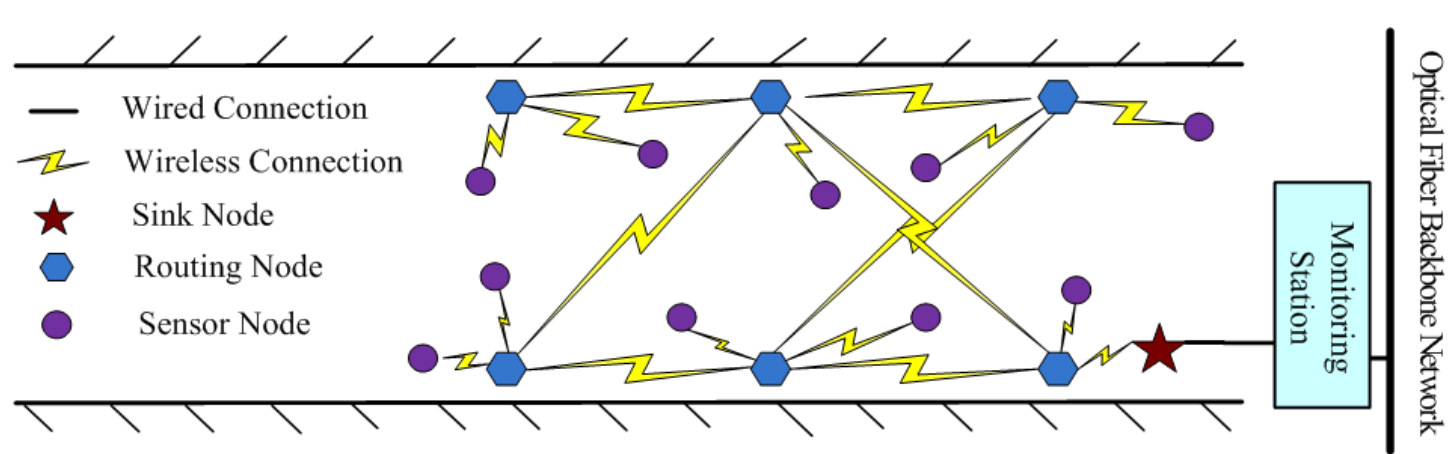
\includegraphics[width=0.7\textwidth]{pictures/wsn_topology.png}
\centering
\caption{Wireless Network Sensor topology in underground corridor example \cite{WSN_monitoring}. }
\label{fig:wsn_topology}
\end{figure}

%WSN routing and topology
Network of wireless connected nodes needs be designed with respect of its maintability. There is need to assume that some nodes may fail during their operation. As the network consits of many nodes, where the number of nodes can be changed during thier operation, there is need to implement actions that will allow them to organize their topology automatically. Even if particural nodes will fail, the rest of nodes should be able to work and maintain communication with remote services. It is the role of implemented routing protocol. There are available solutions that allow network to adapt quickly to the changing environment \cite{WSN_collective}, but in case of statically placed network elements the environment is not changing havily. As it is in common practise, routing nodes stores information about nodes that are used for network purposes in the routing tables. Rounting tables are created with the manner that there are promoted link to nodes that ensure the lowest cost (distance) of packet travel from given node to the sink node. Routing table can have many entries. In case of topology for underground installation there are suggested 3 entries: parent route, minimum route, backup route \cite{WSN_monitoring}. Parent route points to the parent node, minimum route points to the best node in therms of the most energy efficient way to the sink node and backup node that points to the second to the best routing node. Each entry consists of elements such as: number of hops (routing nodes from itself to the sink node), value expressing quality of link of the last communication, flag that describe the role of the entry (parent, minimum, backup route). Routing tables and interconnections between nodes are created during network installation process. The idea is that the sink node that is directly connected to external communication medium creates at first 1-node WSN. Rest of nodes organize themselves in manner that nodes broadcasts their physical and network adresses. Basing on information gathered during installation they are able to determine their position in the network, obtain network address, assign routing table entries and obtain hop number. The network topology can be build up and maintain after WSN installation process \cite{ZigBee_applications}. Nodes are able to pass information to sink node that contains it's routing tables. Thanks to that sink node is able to recreate network topology and then pass the information to the external server. In order to maintain the network there are implemented status messages that contain information about changes in nodes routing tables. They are usually pass through WSN along with data from periodic sensor readings.

%WSN power management
Nodes are equiped with batteries that makes them independent from external power source. In order to save the energy and in order to prolong device live on the battery nodes works in energy efficient modes. In these modes nodes are turned into sleep for certain time. They woke up in order to perform tag readings and transfer the data to the external resources. In order to synchronize their operation, in each cycle the sink node broadcasts the initial message which is used to synchronize all of attached nodes. Power level of nodes batteries are monitored. Nodes can send information about their power level as a repsponce for appropriate request. There can be implemented special routines inside node that can cause sending the information about the low battery level in emergency mode, without any request from the sink node.

%WSN Location management
The crucial for the positioning system is to determine accurately exact position of given reader node inside the underground installations. Without information about readers placement positioning data obtained from them are not usefull. Solution for this problem in WSN positioning systems are solved by manual configuration. Each node have it's own identification number that is a part of it's initial configuration. This number is atteched into their housing also so given nodes can be identified directly during the installation or maintenance work in tunnel. As nodes deployment is regular it is assument in advance what will be the position of the node within the tunnel. In case of sudden failure of some node it is possible to determinate which of the node is broken by it's ID information, and check were the node is placed. WSN network should have possibility to report failure of its nodes. That is why WSN positioning systems are equiped with failure detection and reporting mechanism. Parent nodes like routing nodes against reader nodes, checks if child nodes responds to the requests. In case of having no response from given node for a given amount of subsequent requests then parent node issue status request command to the child node and wait given amount of time. If child node give an answer then it is assumed that the given child node is working correctly. In case of no response from child node, the parent node send information about failure to external service. As the readers nodes are connected stright to the parent node with no routing options then different policy for borken parent node must be applied. If the child node does not reiceve acknowledgement (ACK) frame from it's parent given amount of times then the node increase it's sending power and retrainsmits it's data again. If there is no result of increasing the power then node goes into network setup mode and scan channel to rejoin the network.

%General solution Architecture
Positioning algorithm in WSN positioning system base on mine layout and assume fixed position of nodes. Information about mine layout and nodes position wihin mine is stored in database on server above ground. Data transferred from nodes into acquisition server is a combination of three values: ID of a node, ID of acquried RFID tag in range of RFID reader module of that node, signal power of this RFID tag, and timestamp. Data is being stored in simplified relational database. This positioning system uses algorithm for finding exact position of RFID tag in dwo diamensional space (x, y). In order to do that algorithm search in database for 3 nodes that acquired given tag sinal with the biggest power. Then it uses simple free space electromagnetic waves propagation model \eqref{eq:prop} to compute distance between node and tag.

\begin{equation}
\label{eq:prop}
P_{ri}=\frac{P_t \cdot G_t \cdot G_{ri} \cdot \lambda^2}{4\pi D_i^2}
\end{equation}

Parameters $P_t$ (signal power generated by tag), $G_t$ (tag antenna gain), $G_{ri}$ (node reader antenna gain) and $\lambda$ (electromagnetic wave length) are constant and known. Parameter ${P_{ri}}$ (received signal power on reader's input) is the only variable in the equation that is needed to compute distance from tag to reader. Maximum likelihood estimation method that base on data from three nodes and thier values of reiceved signal power from given tag produces relative position of given tag in (x, y) coordinates. Suggested implementation \cite{WSN_tracking} assume that nodes look for RFID nodes each 10 minutes.
% subsubsection wsn_based_positioning_finding_systems (end)

%drawback of WSN - simplified assumtion about propagation in underground corridors because of wave diffractions on it's walls; - not needed precision of two diamensional space; assumption about RFID tag range (WHAT IS THE RANGE OF RFID). In order to fulfill assumption there is need to put WSN nodes close to each other which higher the costs; - Limited lifetime
%advantages of WSN - wireless nodes with rfid reader modules are cheaper than wired ones (in the same price we can install more nodes)

\section{Localization system choise (system based on beacons)}
* Motivation
* Prototype system description
* Mobile device - system interaction description
** Method of detecting reference points description
** What are the possibilities to improve positioning on your mobile device?
** How could the process of installing a localisation system in a mine look like?
** How the parameters of the environment (corridor height, corridor width, type of rock, type of corridor corridors, presence of other networks operating on similar frequencies (WiFi, GSM (harmonic frequencies)), others) affect reference point signal quality.



\chapter{Mobile device position finding algorithm}
* Algorithm that will make use of chosen localization system and mobile device internal sensors.

\section{Position finding requirements} % (fold)
\label{sec:position_finding_requirements}

* Should repeat and answer requirements stated for localization system.
* example:
** Reading signal and its parameters from reference points;
** Identification of reference points
** Current location presentation on the environment model


% section position_finding_requirements (end)

\section{Simple position finding algorithm implementation} % (fold)
\label{sec:simple_position_finding_algorithm_implementation}

* Simple algorithm will use localization system only (no internal sensors)

% section simple_position_finding_algorithm_implementation (end)

\section{Extended position finding algorithm implementation} % (fold)
\label{sec:extended_position_finding_algorithm_implementation}

* Algorithm will use localization system and internal sensors

% section extended_position_finding_algorithm_implementation (end)

\chapter{Localization system tests}

\section{Tests criteria and assumptions} % (fold)
\label{sec:tests_criteria_and_assumptions}

* Define factors that are important to state if solution is good or not
* Will allow to check if system fulfills requirements
* Test features stated in 'Localization system choise section'

% section tests_criteria_and_assumptions (end)

\section{Tests metodology} % (fold)
\label{sec:tests_metodology}

* Testing environment descipription
* Equimpent used during tests. Example:
** using a representative wifi router, 801.11g techonology, simple circular antenna (eg Minetronics MMG) - for charts.
** using a representative beacon
** dBm signal strength depending on the distance and polarity of the mobile device from the signal source
* Pictures

% section tests_metodology (end)

\section{Tests of system and basic algorithm} % (fold)
\label{sec:tests_of_system_and_basic_algorithm}

* Check if system works with basic algorithm
* Tests in few configurations
* State if some factors have impact on signal quality
* State if some factors have impact on position finding
% section tests_of_system_and_basic_algorithm (end)

\section{Tests of extended algorithm} % (fold)
\label{sec:tests_of_extended_algorithm}

* Capture data that will be base for comparison between simple and extended position finding algorithm accuracy

% section tests_of_extended_algorithm (end)

\section{Experiments results} % (fold)
\label{sec:experiments_results}

* Resluts with analysis

% section experiments_results (end)

\section{Tests summary} % (fold)
\label{sec:tests_summary}

% section tests_summary (end)
\end{document}